\documentclass[11pt,letterpaper]{report}
\usepackage{amssymb,amsfonts,color,graphicx,amsmath,enumerate}
\usepackage{amsthm,hyperref}

\newcommand{\naturals}{\mathbb{N}}
\newcommand{\integers}{\mathbb{Z}}
\newcommand{\complex}{\mathbb{C}}
\newcommand{\reals}{\mathbb{R}}
\newcommand{\mcal}[1]{\mathcal{#1}}
\newcommand{\rationals}{\mathbb{Q}}
\newcommand{\field}{\mathbb{F}}
\newcommand{\Var}{\text{Var}}
\newcommand{\ind}{\mathbbm{1}}
\newcommand{\Cov}{\text{Cov}}
\newcommand{\subg}[1]{\left\|{#1}\right\|_{\psi_2}}
\newcommand{\Lp}[2]{\big\|{#1}\big\|_{L^{#2}}}

\newenvironment{solution}
{\begin{proof}[Solution]}
{\end{proof}}

\voffset=-3cm
\hoffset=-2.25cm
\textheight=24cm
\textwidth=17.25cm
\addtolength{\jot}{8pt}
\linespread{1.3}

\begin{document}
\noindent{\em Liam Hardiman\hfill{May 6, 2020} }
\begin{center}
{\bf \Large 270C - Homework 2}
\vspace{0.2cm}
\hrule
\end{center}
%Exercises: 3.1.4, 3.1.5, 3.1.6, 3.1.7, 3.2.6, 3.3.3, 3.3.5, 3.4.3, 3.4.4, 3.4.5, 3.4.10, 3.5.3, 3.5.7, 3.6.7, 4.4.3, 4.6.4 (just prove (4.22)), 4.7.5
\section*{3.1.4}
Let $X = (X_1, \ldots, X_n)\in \reals^n$ be a random vector with independent, sub-gaussian coordinates $X_i$ that satisfy $E[X_i^2] = 1$. Set $K = \max_i \subg{X_i}$
\begin{enumerate}[(a)]
	\item Show that
	\[
	\sqrt{n}-CK^2 \leq E \|X\|_2 \leq \sqrt{n} + CK^2.
	\]
	
	\begin{proof}
		By Theorem 3.1.1, we have that $\subg{\|X\|_2 - \sqrt{n}} \leq CK^2$ for some absolute constant $C$. In particular, we have that for any $t\geq 0$,
		\[
		\Pr\big[\big|\|X\|_2 - \sqrt{n}\big| > t\big] \leq 2\exp(-t^2/(CK^2)^2).
		\]
		This gives
		\begin{align*}
			E\big[\big|\|X\|_2 - \sqrt{n}\big|\big] &= \int_0^\infty \Pr\big[\big|\|X\|_2 - \sqrt{n}\big| > t\big]\ dt\\
			&\leq \int_0^\infty 2\exp(-t^2/(CK^2)^2)\ dt\\
			&= CK^2\sqrt{\pi}.
		\end{align*}
		Rearranging gives
		\[
		\sqrt{n} - CK^2\sqrt{\pi} \leq E\|X\|_2 \leq \sqrt{n} + CK^2\sqrt{\pi}.
		\]
	\end{proof}

	\item Can $CK^2$ be replaced by $o(1)$?
	\begin{solution}
		
	\end{solution}
\end{enumerate}










\section*{3.1.5}
Deduce from the previous exercise that
\[
\Var(\|X\|_2) \leq CK^4.
\]
\begin{proof}
	We have that
	\begin{align*}
		\Var[\|X\|_2] &= E\left[(\|X\|_2 - E\|X\|_2)^2\right]\\
		&= E\left[(\|X\|_2 - \sqrt{n})^2\right] + 2(\sqrt{n}-E\|X\|_2)E[\|X\|_2-\sqrt{n}] + (\sqrt{n}-E\|X\|_2)^2.
	\end{align*}
	By the previous exercise, this quantity is less than
	\[
	E\left[(\|X\|_2-\sqrt{n})^2\right]+3C^2K^4.
	\]
	Now by theorem 3.1.1, $\|X\|_2-\sqrt{n}$ is sub-Gaussian with norm $K$. Consequently, we can bound its second moment, $E[(\|X\|_2-\sqrt{n})^2] \leq 2K^2$. Putting it all together, we have
	\[
	\Var[\|X\|_2] \leq C^2K^4+ 2K^2.
	\]
\end{proof}










\section*{3.1.6}
Let $X = (X_1, \ldots, X_n)\in \reals^n$ be a random vector with independent coordinates $X_i$ that satisfy $EX_i^2 = 1$ and $EX_i^4 \leq K^4$. Show that
\[
\Var[\|X\|_2] \leq CK^4.
\]
\begin{proof}
	First we claim that $E(\|X\|_2^2-n)^2 \leq K^4n$. This follows from simply expanding $\|X\|_2^4$.
	\begin{align*}
		E(\|X\|_2^2-n)^2 &= E\left[\|X\|_2^4 - n^2\right]\\
		&= \sum_{i=1}^nE[X_i^4] + 2\sum_{i<j}E[X_i^2X_j^2] - n^2\\
		&\leq nK^4 + n(n-1)-n^2\\
		&\leq K^4n.
	\end{align*}
	From this we have
	\begin{align*}
		K^4n &\geq E\left[\left(\|X\|_2^2-n\right)^2\right]\\
		&= E\left[\left(\|X\|_2-\sqrt{n}\right)^2\left(\|X\|_2+\sqrt{n}\right)^2\right]\\
		&\geq nE\left[\left(\|X\|_2-\sqrt{n}\right)^2\right],
	\end{align*}
	so $E(\|X\|_2-\sqrt{n})^2 \leq K^4$. Since the mean minimizes the mean-square error, i.e.
	\[
	\Var[\|X\|_2] \leq E[(\|X\|_2 - c)^2]
	\]
	for all $c\in \reals$, we deduce that $\Var[\|X\|_2] \leq CK^4$.
\end{proof}










\section*{3.1.7}
Let $X = (X_1, \ldots, X_n)\in \reals^n$ be a random vector with independent coordinates $X_i$ with continuous distributions. Assume that the densities of $X_i$ are uniformly bounded by 1. Show that for any $\epsilon>0$, we have
\[
\Pr[\|X\|_2 \leq \epsilon \sqrt{n}] \leq (C\epsilon)^n.
\]
\begin{proof}
	We square and apply the tried and true ``multiply by $\lambda$ and exponentiate'' trick.
	\begin{align*}
		\Pr[\|X\|_2 \leq \epsilon \sqrt{n}] &= \Pr\left[-\frac{1}{\epsilon^2}\|X\|_2^2 \geq -n\right]\\
		&\leq e^{\lambda n}\prod_{i=1}^nE\left[ e^{-\lambda X_i^2/\epsilon^2}\right].
	\end{align*}
	Let's bound those moment generating functions. If $f_i$ is the density of $X_i$, then since $\Lp{f_i}{\infty}\leq 1$ for all $i$, we have
	\begin{align*}
		E\left[e^{-\lambda X_i^2/\epsilon^2}\right] &= \int_\reals e^{-\lambda x^2/\epsilon^2}f_i(x)\ dx\\
		&\leq \int_\reals e^{-\lambda X_i^2/\epsilon^2}\ dx\\
		&= \epsilon\sqrt{\pi/\lambda}.
	\end{align*}
	Combining this with the preceding paragraph gives
	\[
	\Pr[\|X\|_2 \leq \epsilon\sqrt{n}] \leq e^{\lambda n}(\epsilon \sqrt{\pi/\lambda})^n = \epsilon^n(e^\lambda \sqrt{\pi/\lambda})^n.
	\]
	This holds for any value of $\lambda >0$, so the result follows by choosing a value of $\lambda$. Optimizing gives $\lambda = 1/2$, so
	\[
		\Pr[\|X\|_2 \leq \epsilon\sqrt{n}] \leq (\epsilon\cdot \sqrt{2\pi e})^n
	\]
\end{proof}










\section*{3.2.6}
Let $X$ and $Y$ be independent, mean zero, isotropic random vectors in $\reals^n$. Check that
\[
E\|X-Y\|_2^2 = 2n.
\]
\begin{proof}
	I don't have any clever expository things to say here.
	\begin{align*}
		E\|X-Y\|_2^2 &= E[X^tX - X^tY - Y^tX + Y^tY]\\
		&= E[X^tX] - E[X^t]E[Y] - E[Y^t]E[X] + E[Y^tY]\\
		&= 2n.
	\end{align*}
\end{proof}










\section*{3.3.3}
Deduce the following properties from the rotation invariance of the normal distribution.
\begin{enumerate}[(a)]
	\item Consider a random vector $g\sim \mcal{N}(0, I_n)$ and a fixed vector $u\in \reals^n$. Then
	\[
	\langle g, u\rangle \sim \mcal{N}(0, \|u\|_2^2).
	\]
	\begin{proof}
		Let $U$ be a rotation matrix such that $Uu = \|u\|e_1$. That is, $U$ rotates $u$ so that it lies on the first coordinate axis. We then have
		\[
		\langle g, u\rangle = \langle U^tUg, u\rangle = \langle Ug, \|u\|e_1\rangle.
		\]
		By rotation invariance, $Ug\sim \mcal{N}(0, I_n)$. Consequently, the above quantity is $\|u\|\cdot g_1 \sim \mcal{N}(0, \|u\|^2)$ by the definition of the multivariate normal distribution.
	\end{proof}

	\item Consider independent random variables $X_i \sim \mcal{N}(0, \sigma_i^2)$. Then
	\[
	\sum_{i=1}^nX_i\sim \mcal{N}(0, \sigma^2)\quad\text{where}\quad\sigma^2 = \sum_{i=1}^n\sigma_i^2.
	\]
	\begin{proof}
		Consider the vector $u = (\sigma_1, \ldots, \sigma_n)$. If $g\sim \mcal{N}(0, I_n)$, then by part (a) we have that $\langle g, u\rangle \sim \mcal{N}(0, \|u\|^2) = \mcal{N}(0, \sigma^2)$. On the other hand, since each $g_i\sim \mcal{N}(0, 1)$, we have
		\[
		\langle g, u\rangle = \sum_{i=1}^n \sigma_ig_i.
		\]
		The claim follows from the fact that $X_i$ equals $\sigma_ig_i$ in distribution.
	\end{proof}

	\item Let $G$ be an $m\times n$ Gaussian random matrix, i.e. the entries of $G$ are independent $\mcal{N}(0, 1)$ random variables. Let $u\in \reals^n$ be a fixed unit vector. Then
	\[
	Gu\sim \mcal{N}(0, I_m).
	\]
	\begin{proof}
		The $i$-th coordinate of $Gu$ is $\langle g_i, u\rangle$, where $g_i$ is the $i$-th row of $G$. Now $g_i\sim \mcal{N}(0, I_n)$, so $\langle g_i, u\rangle \sim \mcal{N}(0, \|u\|^2) = \mcal{N}(0, 1)$ by part (a) and all the coordinates of $Gu$ are standard normal random variables.\\

		It remains to show that the covariance matrix of $Gu$ is $I_m$. Since $u$ is a unit vector we have
		\begin{align*}
			\Cov(Gu) = E[(Gu)(Gu)^t] = E[G(uu^t)G^t] = E[GG^t].
		\end{align*}
		Now since the entries of $G$ are iid standard normal random variables, $E[GG^t] = I_m$ and the result follows.
	\end{proof}
\end{enumerate}










\section*{3.3.5}
Let $X\sim \mcal{N}(0, I_n)$.
\begin{enumerate}[(a)]
	\item Show that, for any fixed vectors $u,v\in \reals^n$, we have
	\[
	E\langle X, u\rangle \langle X, v\rangle = \langle u, v\rangle.
	\]
	\begin{proof}
		Since $X\sim \mcal{N}(0, I_n)$, we have $E[XX^t] = I_n$. Consequently, we have
		\[
		E\langle X, u\rangle \langle X, v\rangle = E[u^tXv^tX ] = E[u^tXX^tv] = u^tE[XX^t]v = \langle u, v\rangle.
		\]
	\end{proof}

	\item Given a vector $u\in \reals^n$, consider the random variable $X_u = \langle X, u\rangle$. From exercise 3.3.3 we know that $X_u \sim \mcal{N}(0, \|u\|_2^2)$. Check that
	\[
	\Lp{X_u - X_v}{2} = \|u-v\|_2
	\]
	for any fixed vectors $u, v\in \reals^n$.
	\begin{proof}
		By part (a) we have $E[X_uX_v] = \langle u, v\rangle$. Thus,
		\begin{align*}
			\Lp{X_u - X_v}{2}^2 &= E[|X_u  -X_v|^2]\\
			&= E[X_u^2 - 2X_uX_v + X_v^2]\\
			&= \|u\|_2^2 - 2\langle u, v\rangle + \|v\|_2^2\\
			&= \|u-v\|_2^2.
		\end{align*}
	\end{proof}
\end{enumerate}










\section*{3.4.3}
\begin{enumerate}[(a)]
	\item Let $X = (X_1, \ldots, X_n)\in \reals^n$ be a random vector with sub-Gaussian coordinates $X_i$. Show that $X$ is a sub-Gaussian random vector.
	\begin{proof}
		We use the moment characterization of sub-Gaussian random variables. Since each $X_i$ is sub-Gaussian, $\Lp{X_i}{p}\leq K_i\sqrt{p}$ for constants $K_i$ and all $p\geq 1$. We then have
		\begin{align*}
			\Lp{\langle X, x\rangle}{p} &= \Lp{\sum_{i=1}^n x_iX_i}{p}\\
			&\leq \sum_{i=1}^n|x_i|\cdot \Lp{X_i}{p}\\
			&\leq \left(\sum_{i=1}^n|x_i|\cdot K_i\right)\sqrt{p},
		\end{align*}
		so $\langle X, x\rangle$ is sub-Gaussian.
	\end{proof}

	\item Find an example of a random vector $X$ with
	\[
	\subg{X} \gg \max_{i\leq n}\subg{X_i}.
	\]
	\begin{solution}
		Let $\xi$ be any real-valued sub-Gaussian random variable and consider the random vector $X = (\sqrt{n}\xi, \ldots, \sqrt{n}\xi)\in \reals^n$. $X$ is sub-Gaussian by part (a). We clearly have
		\[
		\max_{i\leq n}\subg{X_i} = \subg{\sqrt{n}\xi} = \sqrt{n}\cdot \subg{\xi}.
		\]
		On the other hand, we have
		\begin{align*}
			\subg{X} &\geq \subg{\left\langle X, \frac{1}{\sqrt{n}}\mathbf{1}\right\rangle}\\
			&= \subg{\sum_{i=1}^n\sqrt{n}\xi\cdot \frac{1}{\sqrt{n}}}\\
			&= n\cdot \subg{\xi},
		\end{align*}
		which is $\omega(\max_{i\leq n}\subg{X_i})$.
	\end{solution}
\end{enumerate}










\section*{3.4.4}
Let $X\in \reals^n$ be a random vector with coordinate distribution. That is, $X$ is uniformly distributed in the set $\{\sqrt{n}e_i: i = 1, \ldots n\}$. Show that
\[
\subg{X}\asymp \sqrt{\frac{n}{\log n}}.
\]
\begin{proof}
	
\end{proof}










\section*{3.4.5}
Let $X$ be an isotropic random vector supported in a finite set $T\subseteq \reals^n$. Show that in order for $X$ to be sub-Gaussian with $\subg{X}= O(1)$, the cardinality of the set must be exponentially large in $n$:
\[
|T|\geq e^{cn}.
\]
\begin{proof}
	
\end{proof}










\section*{3.4.10}
Let $X = (X_1, \ldots, X_n)\in \reals^n$ be random vector with independent, sub-Gaussian coordinates $X_i$ that satisfy $EX_i^2=1$. Then
\[
\subg{\|X\|_2 - \sqrt{n}}\leq CK^2,
\]
where $K = \max_i\subg{X_i}$ and $C$ is an absolute constant. Show that this concentration inequality may not hold for a general isotropic sub-Gaussian random vector $X$.
\begin{proof}
	
\end{proof}










\section*{3.5.3}
Let $A = (a_{ij})$ be a symmetric real $n\times n$ matrix. Suppose that $A$ is either positive semidefinite or has zero diagonal. Assume that, for any numbers $x_i\in \{-1, 1\}$ we have
\begin{equation}\label{groth_hyp}
\bigg|\sum_{i,j}a_{ij}x_ix_j\bigg|\leq 1.
\end{equation}
Then, for any Hilbert space $H$ and any vectors $u_i,v_j\in H$ satisfying $\|u_i\|=\|v_j\| = 1$, we have
\[
\bigg|\sum_{i,j}a_{ij}\langle u_i, v_j\rangle\bigg|\leq 2K,
\]
where $K$ is the absolute constant from Grothendieck's inequality.
\begin{proof}
	Note that (\ref{groth_hyp}) can be written as $|\langle Ax, x\rangle|\leq 1$. Observe the following polarization identity.
	\begin{align*}
		\left\langle A\left(\frac{x+y}{2}\right),\frac{x+y}{2}\right\rangle - \left\langle A\left(\frac{x-y}{2}\right),\frac{x-y}{2}\right\rangle &= \frac{1}{4}[\langle A(x+y), x+y\rangle -  \langle A(x-y), x-y\rangle]\\
		&= \langle Ax, y\rangle.
	\end{align*}
	Then, if we set $u = \frac{1}{2}(x+y)$ and $v = \frac{1}{2}(x-y)$, we have.
	\begin{equation}\label{groth_goal}
	|\langle Ax, y\rangle|  \leq |\langle Au,u\rangle| + |\langle Av, v\rangle|
	\end{equation}
	Unfortunately, the vectors $u$ and $v$ are in $\{-1, 0, 1\}^n$, not $\{-1, 1\}^n$. If we could show that our hypothesis holds for vectors of this form as well, then the above quantity would be less than 2 and we could apply Grothendieck's inequality. (So far we haven't used the symmetry of $A$.)\\

	(The idea for this part comes from a stackexchange \href{https://math.stackexchange.com/questions/2739932/symmetric-grothendieck-inequality}{post}) We claim that, under our hypotheses, for any $I\subset [n]$ and any $x\in \{-1, 1\}^n$ we have
	\[
	-1 \leq \sum_i a_{ii}+ \sum_{i\neq j\in I}a_{ij}x_ix_j\leq 1.
	\]
	To see this, fix a subset $I\subseteq [n]$ and some vector $y\in \{-1, 1\}^n$. Now consider the set of vectors $x\in \{-1, 1\}^n$ that agree with $y$ on $I$. There are $M = 2^{n - |I|}$ such vectors. For any such vector, we have by hypothesis
	\[
	-1 \leq \sum_{i}a_{ii} + \sum_{i\neq j}a_{ij}x_ix_j\leq 1.
	\]
	Now let's add all $M$ of these inequalities together. Since each vector is in $\{-1, 1\}^n$, the diagonal term $\sum_{i}a_{ii}$ will appear in each of them. Since each of these vectors agrees on $I$, we'll get a $\sum_{i\neq j\in I}a_{ij}x_ix_j$ for each of them. Now for every choice of coordinates outside of $I$, there is an ``opposite'' choice to make by flipping each coordinate outside of $I$. These sums cancel with each other, leaving only the diagonal and $I$ terms. This gives
	\[
	-M\leq M\sum_ia_{ii} + M\sum_{i\neq j\in I}a_{ij}x_ix_j\leq M.
	\]
	Dividing through by $M$ establishes the claim. (I don't think we used the symmetry of $A$ anywhere here.)\\

	Now let's return to our problem. Consider the case where $A$ has zeros on its diagonal and let $u\in \{-1, 0, 1\}^n$. Let $I$ be the support of $u$ and let $\tilde{u}$ the vector that agrees with $u$ on the support of $u$ and is 1 elsewhere. By our claim we have
	\[
	\langle Au, u\rangle = \sum_{i\neq j}a_{ij}u_iu_j = \sum_{i\neq j\in I}a_{ij}\tilde{u}_i\tilde{u}_j.
	\]
	The last quantity is less than 1 in absolute value by hypothesis, so (\ref{groth_goal}) is less than 2 and we can apply Grothendieck (still haven't used symmetry). Now suppose that $A$ is PSD and let $u\in \{-1, 0, 1\}^n$. In this case we have $0\leq \langle Au, u\rangle$, so we only need to show that $\langle Au, u\rangle \leq 1$. Since $A$ is PSD, its diagonal entries are nonnegative. Letting $I$ and $\tilde{u}$ be as in the zero-diagonal case, we have
	\[
	\langle Au, u\rangle= \sum_{i\in I}a_{ii} + \sum_{i\neq j}a_{ij}u_iu_j \leq \sum_ia_{ii} + \sum_{i\neq j\in I}a_{ij}\tilde{u}_i\tilde{u}_j.
	\]
	The last quantity is less than 1 in absolute value, so again we can apply Grothendieck. (I don't think we used symmetry at any point here.)

\end{proof}










\section*{3.5.7}
\newcommand{\sign}{\text{sign}}
\section*{3.6.7}
Consider a random vector $g\sim \mcal{N}(0, I_n)$. Show that for any fixed vectors $u, v\in S^{n-1}$ we have
\[
E[\sign\langle g, u\rangle \sign \langle g, v\rangle] = \frac{2}{\pi}\arcsin\langle u, v\rangle.
\]
\begin{proof}
	\begin{figure}\label{groth}
		\centering
			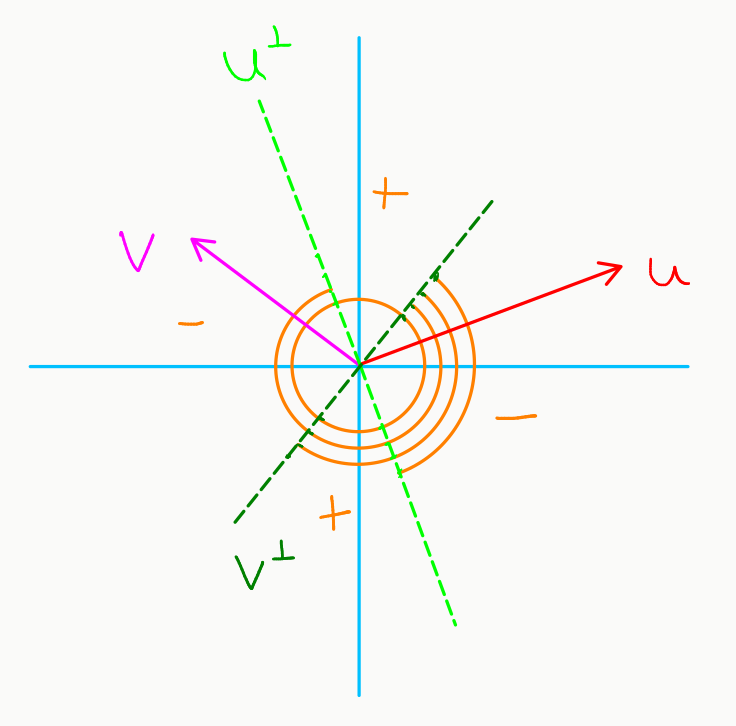
\includegraphics[scale=0.5]{groth.PNG}
			\caption{An orange ``+'' or ``-'' indicates the sign of $\langle g, u\rangle\langle g, v\rangle$ for $g$ in the indicated region.}
	\end{figure}
	By rotation invariance, we can assume that $g$ lies in the plane determined by $u$ and $v$. As shown in Figure 1, $\langle g, u\rangle\langle g, v\rangle$ is positive if and only if the angles between $g$ and $u$ and between $g$ and $v$ are both acute or both obtuse. Call the event that $g$ satisfies this condition $E$ and let $\theta$ be the angle between $u$ and $v$. By the rotation invariance of the multivariate normal distribution, the angle $\langle g, u\rangle/\|g\|_2$ is a uniform random variable. We then have
	\begin{align*}
		E[\sign\langle g, u\rangle \sign \langle g, v\rangle] &= \Pr[E] - \Pr[E^C]\\
		&= \frac{2\pi -2\theta}{2\pi} - \frac{2\theta}{2\pi}\\
		&= \frac{2}{\pi}\left(\frac{\pi}{2}-\theta\right)\\
		&= \frac{2}{\pi}\arcsin\langle u, v\rangle.
	\end{align*}
\end{proof}










\section*{4.4.3}
Let $A$ be an $m\times n$ matrix and $\epsilon\in [0, 1/2)$.
\begin{enumerate}[(a)]
	\item Show that for any $\epsilon$-net $\mcal{N}$ of the sphere $S^{n-1}$ and any $\epsilon$-net $\mcal{M}$ of the sphere $S^{m-1}$, we have
	\begin{equation}\label{epsnet1}
		\sup_{x\in \mcal{N}, y\in \mcal{M}}\langle Ax, y\rangle \leq \|A\|\leq \frac{1}{1-2\epsilon}\cdot \sup_{x\in \mcal{N}, y\in \mcal{M}}\langle Ax, y\rangle.
	\end{equation}

	\begin{proof}
		The lower bound trivially follows from the fact that
		\[
		\|A\| = \max_{x\in S^{n-1}, y\in S^{m-1}}\langle Ax, y\rangle.
		\]
		As for the upper bound, fix vectors $x\in S^{n-1}$ and $y\in S^{m-1}$ that realize the operator norm bound: $\|A\| = \langle Ax, y\rangle$. Let $x_0\in \mcal{N}$ and $y_0\in \mcal{M}$ be such that $\|x-x_0\|_2 \leq \epsilon$ and $\|y-y_0\|_2\leq \epsilon$. We have
		\begin{align*}
			|\langle Ax, y\rangle - \langle Ax_0, y_0\rangle| &= |\langle Ax, y-y_0\rangle + \langle A(x-x_0), y_0\rangle|\\
			&\leq \|A\|\|x\|_2\|y-y_0\|_2 + \|A\|\|(x-x_0)\|_2\|y_0\|_2\\
			&\leq 2\epsilon\|A\|.
		\end{align*}
		By the triangle inequality we then have
		\begin{align*}
			|\langle Ax_0, y_0\rangle| &\geq \|A\| - 2\epsilon\|A\|,
		\end{align*}
		which gives the desired upper bound.
	\end{proof}

	\item Moreover, if $m=n$ and $A$ is symmetric, show that
	\[
	\sup_{x\in \mcal{N}}|\langle Ax, x\rangle|\leq \|A\| \leq \frac{1}{1-2\epsilon}\cdot \sup_{x\in \mcal{N}}|\langle Ax, x\rangle|.
	\]
	\begin{proof}
		Use the exact same argument from part (a) since the operator norm of a symmetric matrix $A$ is given by
		\[
		\|A\| = \sup_{x\in S^{n-1}}\langle Ax, x\rangle.
		\]
	\end{proof}
\end{enumerate}










\section*{4.6.4}

\section*{4.7.5}


\end{document}